\documentclass{article}
\usepackage{ctex}
\usepackage{graphicx}
\usepackage{float}
\graphicspath{{figures/},{pics/}}

\title{针对用户贷款情况进行预测}
\author{吴浩邦,刘俊麟,祝瑞}
\begin{document}

\maketitle

\begin{abstract}
本次数据挖掘导论的期末作业我们选择的是DataCastle中的“用户贷款风险预测”。实验是根据题目所给出的每个用户的特征如用户的基本属性、银行流水、信用卡账单记录等等来建立准确的风险控制模型,以此来预测用户是否会逾期还款。由于数据规模较大,包含7万条数据,故先将数据进行特征值的筛选,而后使用Xgboost进行模型训练。
\end{abstract}

\section{赛题分析}
赛题内容:融360与平台上的金融机构合作,提供了近7万贷款用户的基本身份信息、消费行为、银行还款等数据信息,需要参赛者以此建立准确的风险控制模型,来预测用户是否会逾期还款。
提供数据:参赛者可用的训练数据包括用户的基本属性user\textunderscore info.txt、银行流水记录bank\textunderscore detail.txt、用户浏览行为browse\textunderscore history.txt、信用卡账单记录bill\textunderscore detail.txt、放款时间loan\textunderscore time.txt,以及这些顾客是否发生逾期行为的记录overdue.txt。(注意:并非每一位用户都有非常完整的记录,如有些用户并没有信用卡账单记录,有些用户却没有银行流水记录。)
分析:题目是对用户进行预测,预测是否会逾期还款,并且通过题中给定的数据进行预测。题中提供了六个数据基本属性、银行流水记录、用户浏览行为、信用卡账单记录、放款时间;训练数据中提供顾客是否发生逾期行为的记录,测试数据中提供需要预测的顾客编号。通过对已有数据可视化并进行特征提取,判断哪些数据与逾期行为有关联,选择适应数据进行模型训练。并且用相应数据预测未知顾客的逾期行为。

\section{数据初始化分析}

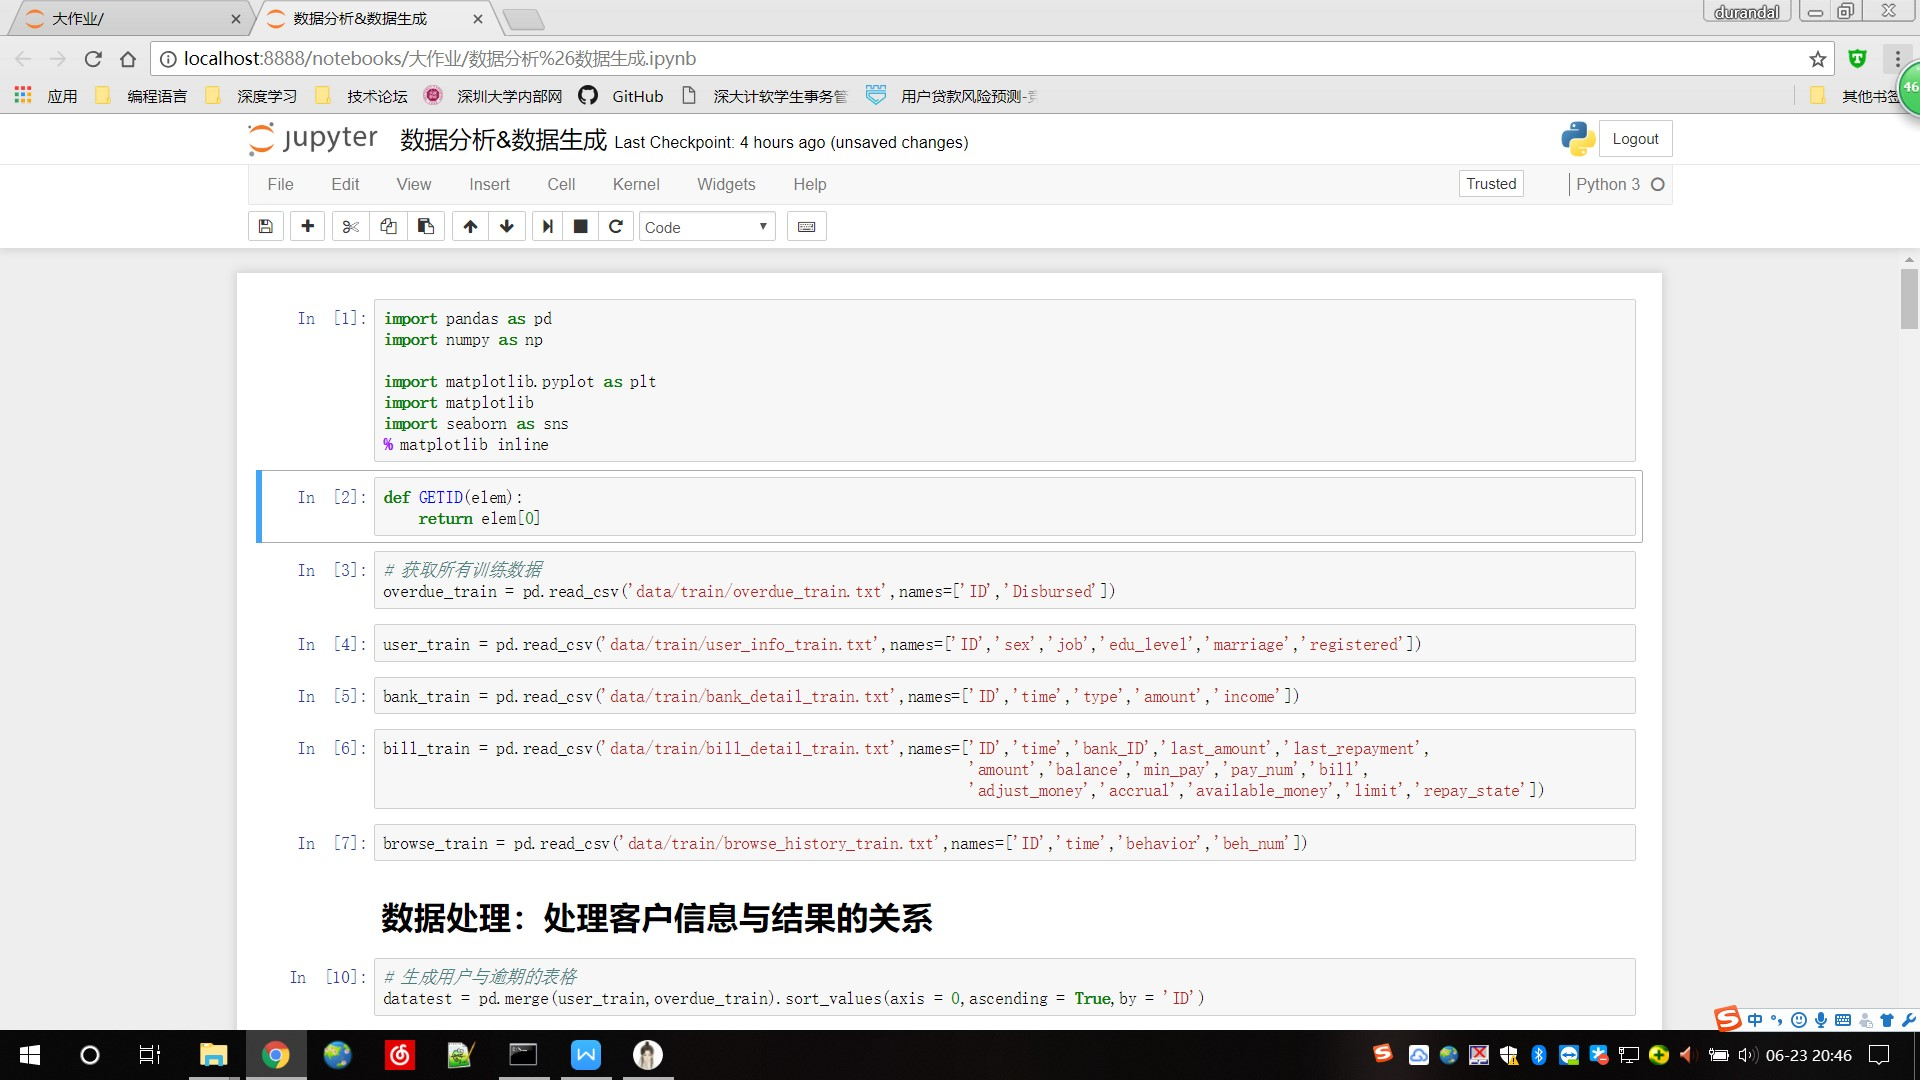
\includegraphics[scale=0.3]{图一}
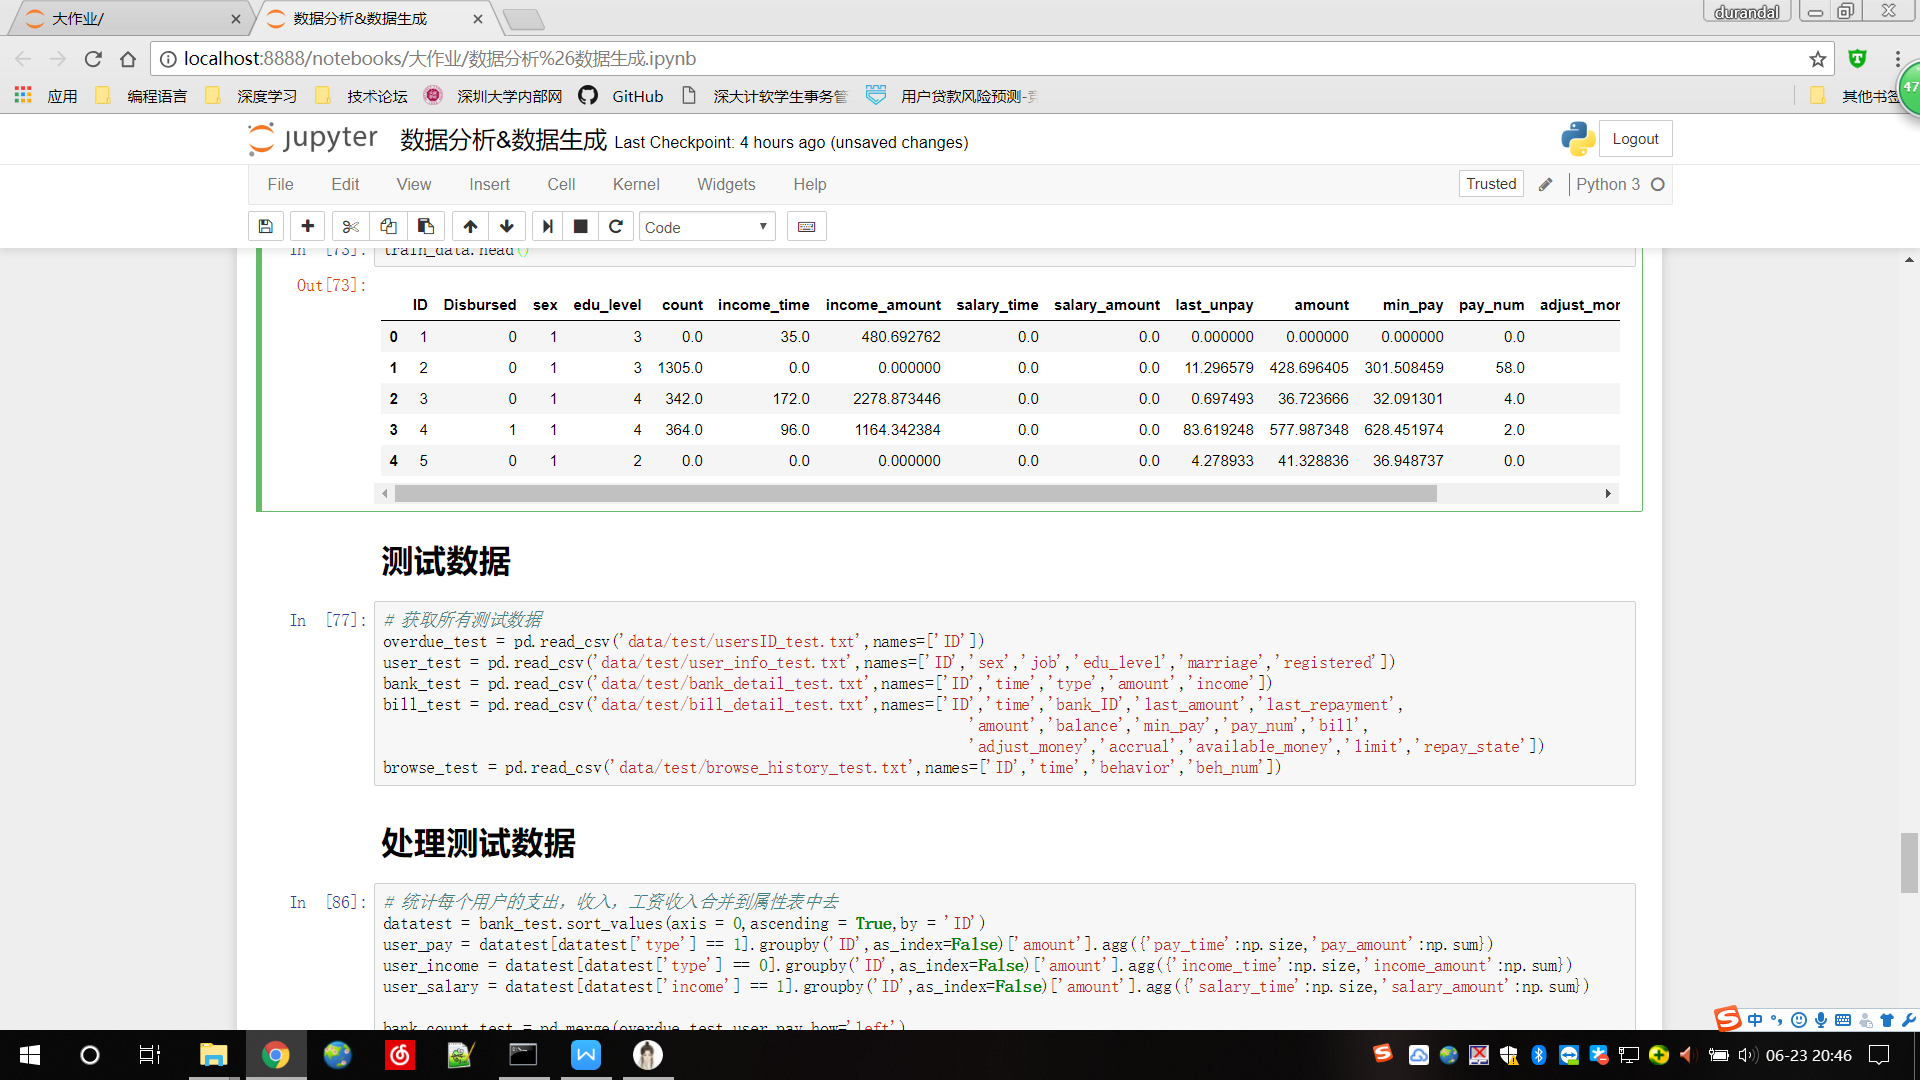
\includegraphics[scale=0.3]{2}

\section{数据思路}
\subsection{基本思路}
对题中提供的四个训练数据:基本属性、银行流水记录、用户浏览行为、信用卡账单记录选取全部或者部分进行按编号分组生成的数据集,并与是否发生逾期行为的记录进行合并,最后对合并后的数据集进行按逾期行为分组绘图,并通过可视化数据进行特征提取。

\subsection{用户基本属性}
\#生成用户与逾期行为表格
\\datatest = pd.merge(user\textunderscore train,overdue\textunderscore train).sort\textunderscore values(axis = 0,ascending = True,by = 'ID') 
\\ \#计算每一个因素的逾期率
\\ \#计算性别与逾期行为几率(以此类推往下)
\\ sex\textunderscore overdue = 
datatest.groupby('sex',as\textunderscore index=False)['Disbursed'].agg({'count':np.size,'num':np.sum})
sex\textunderscore overdue['over\textunderscore rate'] = sex\textunderscore overdue['num']/sex\textunderscore overdue['count']
\\ \#计算职业与逾期行为几率
\\ \#计算教育程度与逾期行为几率
\\ \#计算婚姻状况与逾期行为几率
\\ \#计算户口与逾期行为几率

\subsection{银行流水记录}

\#统计每个用户的支出,收入,工资收入合并到属性表中去
\\ \#计算用户支出总量
\\user\textunderscore pay = datatest[datatest['type'] ==
1].groupby('ID',as\textunderscore index=False)['amount'].agg({'pay\textunderscore time':np.size,'pay\textunderscore amount':np.sum})
\\ \#计算用户收入总量
\\ \#计算用户薪水总量
\\ \#合并所有总量以及逾期行为并把无数据的用户的数据置零
\\bank\textunderscore count = pd.merge(overdue\textunderscore train,user\textunderscore pay,how='left')

\subsection{用户浏览行为}
\#按照用户编号分组计算浏览次数
\\browse\textunderscore data = 
browse\textunderscore train.groupby('ID',as\textunderscore index=False)['ID'].agg({'count':np.size})
\\ \#合并总量以及逾期行为
\\browse\textunderscore data = pd.merge(overdue\textunderscore train,browse\textunderscore data,how='left').sort\textunderscore values
(axis = 0,ascending = True,by = 'ID')
browse\textunderscore data = browse\textunderscore data.fillna(0)



\subsection{信用卡账单记录}
\#获取上期未还金额,计算方法:上期未还金额=上期账单-上期还款
\\datatest = bill\textunderscore train.copy()
\\ \#上期未还金额不可为负
\\f = lambda x:x['last\textunderscore amount']-x['last\textunderscore repayment'] 
if x['last\textunderscore amount']-x['last\textunderscore repayment']>0 else 0
datatest['last\textunderscore unpay'] = datatest.apply(f,axis=1)
\\ \#计算上期未还金额
\\ \#计算信用卡额度
\\ \#计算本期最低还款额度
\\ \#计算消费笔数
\\ \#计算调整金额总数
\\ \#计算循环利息
\\ \#计算预借现金额度
\\ \#合并总量以及逾期行为
\\bill\textunderscore data = pd.merge(overdue\textunderscore train,last\textunderscore unpay,how='left').sort\textunderscore values(axis = 0,ascending = True,by = 'ID')


\section{数据特征值}
选择训练数据:性别,教育程度,婚姻状况,收入总次数,收入金额总数,工资收入次数,工资收入总金额,浏览总数,信用卡额度,本期最低还款额,消费笔数,调整金额,利息,预借现金额度。
以下为选择依据:

选择思路:对于每个数据都进行逾期行为的概率进行统计并绘图。
\begin{figure}[h] 
\centering 
\includegraphics[scale=0.3]{一}
\caption{性别、工作、教育程度、婚姻状况以及户籍的逾期行为比率柱形图}

\leftline{银行流水记录:}
\leftline{\#支出,收入,工资收入与是否逾期的关系}

\end{figure}

\begin{figure}[h]
\centering 
\includegraphics[scale=0.3]{二}
\includegraphics[scale=0.3]{三}
\caption{付款次数和付款总额的逾期行为散点图}
\end{figure}

\begin{figure}[h]
\includegraphics[scale=0.5]{四}
\caption{薪水次数和薪水总额的逾期行为散点图}
\leftline{用户浏览行为:}
\#浏览次数与逾期行为
\end{figure}


\begin{figure}[h]
\centering 
\includegraphics[scale=0.5]{五}
\caption{浏览次数与逾期行为散点图}
\leftline{信用卡账单记录:}
上期未还,信用卡额度,本期最低还款,消费总笔数,调整金额,循环利息,预借现金额度与是否逾期的关系
\end{figure}

\begin{figure}[h]
\includegraphics[scale=0.3]{六}
\caption{上期未还、信用卡额度和本期最低还款与逾期行为散点图}
\end{figure}

\begin{figure}[h]
\includegraphics[scale=0.3]{七}
\caption{消费总笔数、调整金额、循环利息与逾期行为散点图}
\end{figure}

\begin{figure}[h]
\centering
\includegraphics[scale=0.3]{八}
\caption{预借现金额度与逾期行为散点图}
\end{figure}

\section{实验结果}

使用xgboost算法对训练数据进行训练,使用生成的模型对测试数据进行预测,预测出每个用户的逾期率,并且提交结果得出比赛成绩。

\begin{figure}[h]
\centering
\includegraphics[scale=0.3]{九}
\caption{xgboost算法数据特征关联结果}

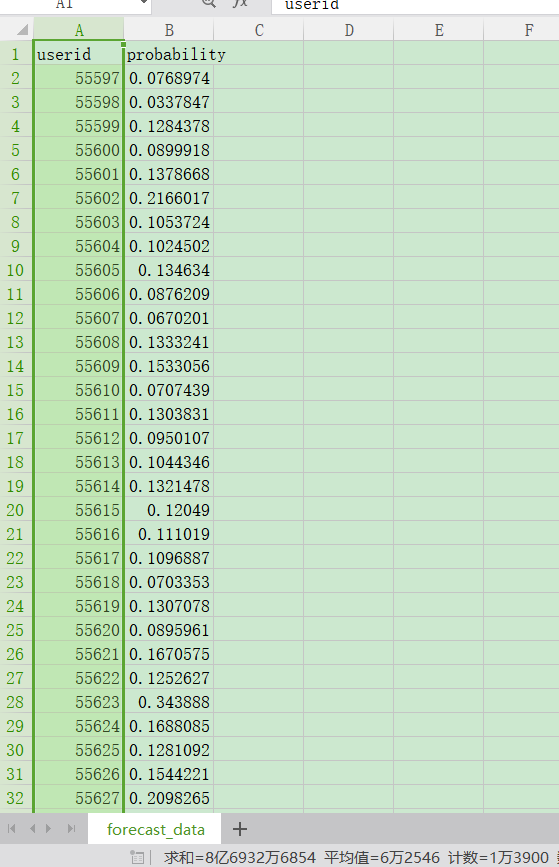
\includegraphics[scale=0.3]{十}
\caption{生成预测百分比}

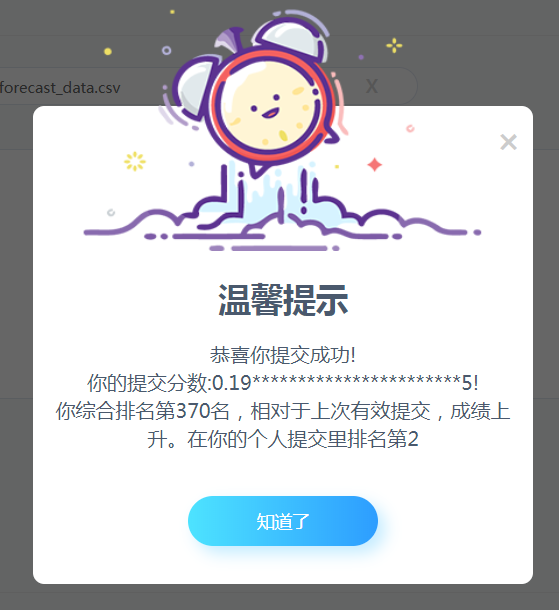
\includegraphics[scale=0.5]{十一}

\includegraphics[scale=0.5]{十二}
\caption{竞赛成绩}

\end{figure}

\section{总结}
在数据分析中,我们先是查阅了大量的有关xgboost的原理文献,并对比xgboost所在的参数,如树的最大深度max\textunderscore depth)、随机森林数的数量(n\textunderscore estimators等等进行一步步分析,其中收获最大的就是了解了xgboost的并行原理,它可以很“简单粗暴”的得到我们想要的结果,这在我以后应用数据挖掘中提到大量的帮助!
根据后期查阅到的知识,xgboost仅仅只能对单模型的数据具有快速强大的作用,并且需要对特征值进行融合,这一点我们虽然有做,但是没有排名前面融合的好。除了xgboost的特征融合,其实还有mic加权融合这种用不同模型,或者不同特征集、不同的样本集、不同的模型)的结果融合,可以有效的避免过拟合。

\end{document}




